%% TODAES draft for Virtuoso-Agent.
%% Build from this directory:
%%   pdflatex main.tex
%%   bibtex main
%%   pdflatex main.tex
%%   pdflatex main.tex

\documentclass[acmsmall,review,anonymous]{acmart}

\usepackage{booktabs}
\usepackage{array}
\usepackage{tabularx}
\usepackage{makecell}
\usepackage{xcolor}
\usepackage{graphicx}
\usepackage{tikz}
\usetikzlibrary{arrows.meta,positioning,fit,calc,shapes.geometric}

\settopmatter{printacmref=false,printccs=false,printfolios=true}
\graphicspath{{figs/}}

\newcommand{\framework}{Virtuoso-Agent}
\newcommand{\bridge}{SafeBridge}
\newcommand{\pass}{\textsc{Pass}}
\newcommand{\fail}{\textsc{Fail}}
\newcommand{\todo}[1]{\textcolor{red}{\textbf{[TODO:} #1\textbf{]}}}
\newcommand{\metric}[1]{\texttt{#1}}

\title{\framework: An NDA-Safe Closed-Loop LLM Framework for Analog Circuit Sizing in Industrial EDA Flows}

\author{Anonymous Author(s)}
\affiliation{%
  \institution{Submission under review}
  \city{}\country{}}
\email{anonymous@submission}
\renewcommand{\shortauthors}{Anonymous}

\begin{document}

\begin{abstract}
Large language models (LLMs) can propose circuit-sizing decisions, but
industrial analog design flows cannot simply expose foundry process-design-kit
(PDK) content, proprietary schematic details, absolute simulation paths, or
license-bound tool state to a cloud endpoint. This paper presents
\framework, an NDA-safe closed-loop framework that lets LLMs optimize
analog circuits through Cadence Virtuoso, Maestro, and Spectre while
returning only scrubbed topology intent, numeric simulation metrics,
operating-point summaries, and scoped writeback status. The framework
combines a two-sided whitelist around SKILL entry points, PDK/path/model
scrubbing, Maestro setup/writeback recipes, result readback, JSON action
contracts, and best-so-far preservation. We evaluate eleven LLM checkpoints
from the same all-ones reset protocol on two real closed-loop tasks: a
20 GHz LC-VCO tuning-curve sizing task and a differential two-stage op-amp
AC/DC sizing task. On the LC-VCO task, 8 of 11 models pass within the
15-iteration budget; on the op-amp task, 6 of 11 pass. The results show
that model quality differs sharply once the loop requires tool discipline,
bias reasoning, and specification repair, and that an NDA-safe EDA boundary
can still provide enough sanitized feedback for successful analog sizing.
\end{abstract}

\keywords{LLM agents, analog circuit sizing, EDA automation, Cadence Virtuoso,
Maestro, Spectre, NDA-safe design automation, LLM4EDA}

\maketitle

\begin{figure}[t]
  \centering
  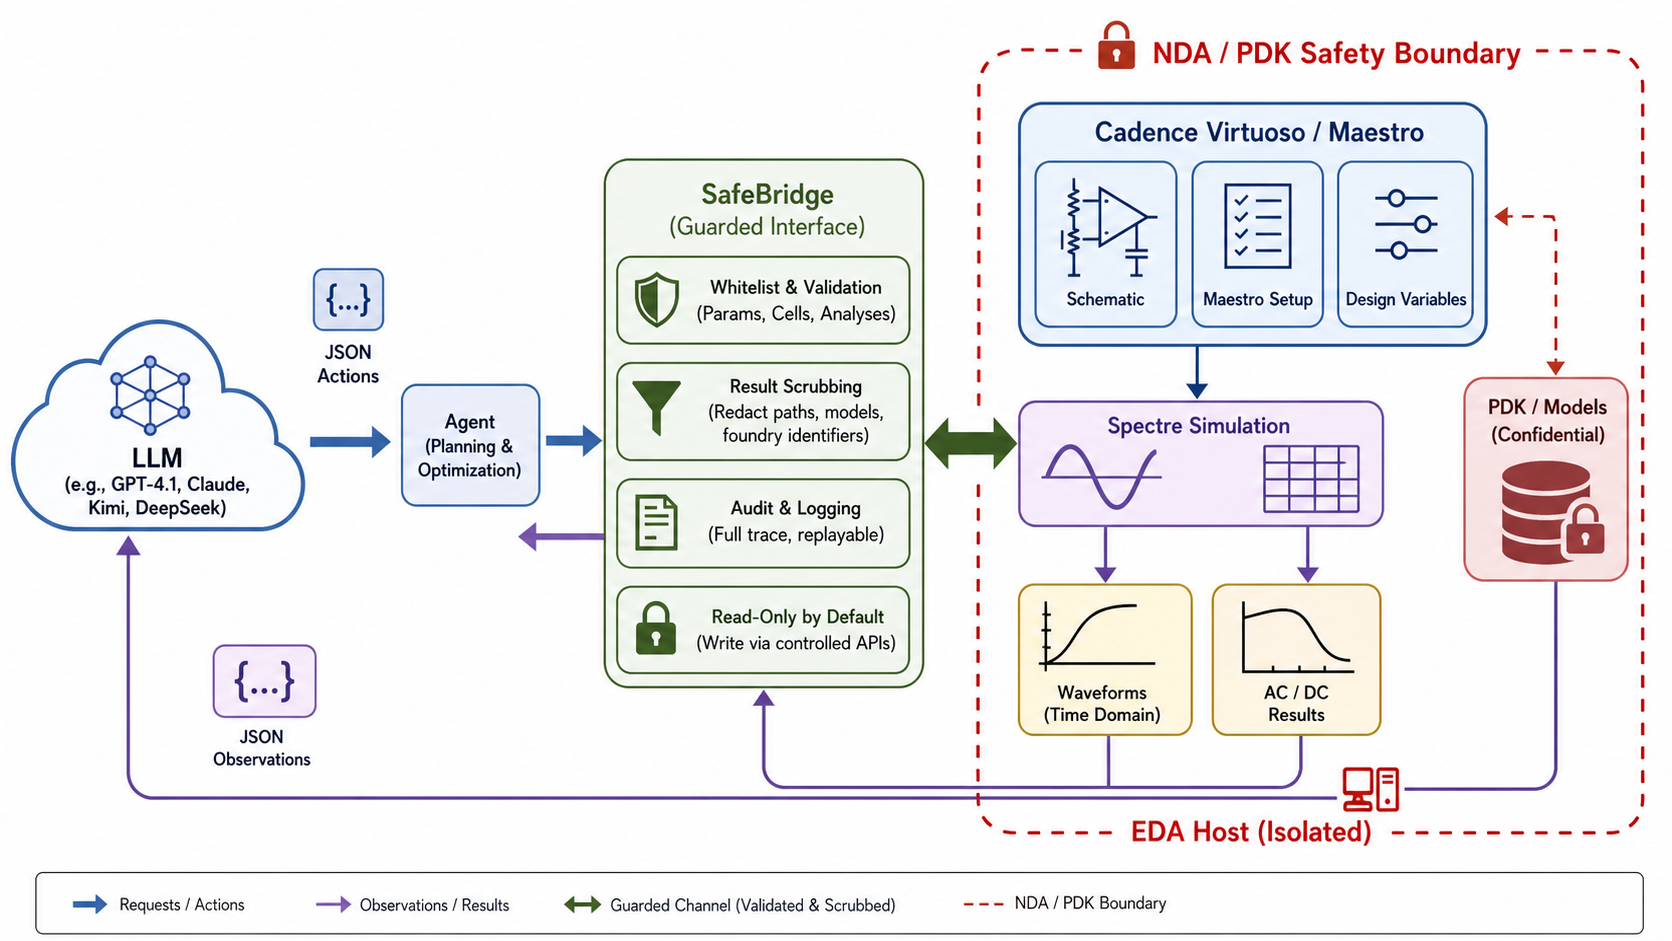
\includegraphics[width=\linewidth]{virtuoso_agent_overview.png}
  \caption{Conceptual overview of \framework. The LLM sees JSON actions and
  scrubbed observations. Foundry PDK content, Maestro state, simulator raw
  paths, and proprietary model details remain inside the isolated EDA host.}
  \label{fig:teaser}
\end{figure}

\section{Introduction}
\label{sec:intro}

LLM-driven EDA loops are useful only when the tool boundary is as carefully
engineered as the prompt. Recent digital and HLS systems use compiler,
synthesis, or simulation feedback to refine LLM-generated artifacts
\cite{autochip,hlsrewriter,c2hlsc,lhs,confibench}. Analog circuit sizing is a
natural next target because SPICE simulation provides a direct numerical
oracle. However, the analog case introduces a deployment constraint that is
not a minor implementation detail: a real foundry-bound Virtuoso flow contains
PDK model cards, proprietary cell names, private schematic hierarchy, absolute
host paths, and license-bound simulation state that cannot be sent to a cloud
LLM.

Existing analog LLM work has made rapid progress on code generation, sizing,
and benchmark design \cite{analogcoder,adollm,eesizer,anaflow,ledro,autosizer,
analogsage,analoggym}. The missing systems question is how to let a frontier
model use the feedback it needs without crossing an NDA boundary. Open-PDK
benchmarks and on-premise small-model deployments are valuable, but they leave
two practical questions unanswered for industrial users: can cloud LLMs be
connected to a real Virtuoso/Maestro loop without leaking PDK content, and how
should models be compared when every run must start from the same documented
EDA state?

This paper argues that the right unit of contribution is not another
standalone prompt or a claim that an LLM is a circuit designer. The unit is a
reproducible, safety-bounded analog sizing substrate. \framework{} wraps the
Cadence SKILL and OCEAN interface with a Python agent, a return-path scrubber,
per-project design-variable whitelists, structured Maestro setup recipes,
simulation-result readback, and a strict JSON action contract. The LLM can
propose numeric design variables and reason over sanitized topology and
operating-point summaries, but it cannot browse arbitrary libraries, read raw
PDK model files, or receive unsanitized simulator paths.

We make four contributions:
\begin{enumerate}
  \item We introduce an NDA-safe closed-loop architecture for LLM-driven analog
  sizing in Virtuoso/Maestro flows, including the trust boundary, whitelist
  layers, scrubbed readback, and scoped writeback protocol.
  \item We define a fair benchmark protocol that resets each model to the same
  initial design-variable state, runs the same Maestro tests, and preserves
  the best numeric point even when no hard-pass point is found.
  \item We report an eleven-model comparison on two circuit classes: an LC-VCO
  tuning-curve task and a two-stage op-amp AC/DC task.
  \item We provide a failure taxonomy showing where closed-loop analog agents
  break: contract violations, missing tool discipline, wrong bias-scale
  reasoning, insufficient use of operating-point evidence, and simulator
  result-generation failures.
\end{enumerate}

\section{Related Work}
\label{sec:related}

\subsection{LLMs in EDA}

LLM4EDA systems have been most visible in digital RTL, HLS, and code-oriented
flows, where the feedback loop can be closed with compiler and synthesis
diagnostics. AutoChip, HLSRewriter, C2HLSC, LHS, and ConfiBench demonstrate
this pattern in TODAES-style settings \cite{autochip,hlsrewriter,c2hlsc,lhs,
confibench}. Those works motivate the central premise of this paper: LLMs
become more useful when the EDA tool is in the loop and the feedback is
machine-checkable.

\subsection{LLMs for analog design}

Analog LLM work has moved from netlist/code generation toward sizing and
workflow automation. AnalogCoder and AnalogCoder-Pro focus on analog circuit
generation and optimization \cite{analogcoder,analogcoderpro}. ADO-LLM,
EEsizer, AnaFlow, LEDRO, AutoSizer, and AnalogSAGE explore LLM-aided sizing,
multi-agent search, memory, and optimization strategies
\cite{adollm,eesizer,anaflow,ledro,autosizer,analogsage}. AnalogGym provides
an open benchmark suite for LLM-driven analog sizing \cite{analoggym}. These
efforts establish that LLMs can participate in analog design loops; our
contribution is complementary, because we target the safety and reproducibility
boundary required by foundry-bound Virtuoso/Maestro deployment.

\subsection{NDA-constrained deployment}

Two broad strategies can address NDA-constrained analog LLM use. One is to
move inference inside the trusted environment, as in on-premise small-model
approaches such as AnalogAgent \cite{analogagent}. The other is to keep cloud
models outside the trusted environment and strictly control what crosses the
boundary. \framework{} takes the second path. It does not claim to remove the
need for local EDA licenses or foundry access; instead, it defines a scrubbed
bridge that lets external models see enough evidence to optimize without
seeing the confidential artifacts that produced the evidence.

\section{Framework}
\label{sec:framework}

\subsection{Closed-loop flow}

\framework{} is organized around a simple loop. The LLM proposes a JSON action
containing design-variable updates. The Python agent validates the action,
writes allowed variables into Maestro, triggers simulation, reads back numeric
results, computes pass/fail status against the specification, and returns a
scrubbed feedback packet. The loop stops when all hard-pass specifications are
met or when the iteration budget is exhausted. If the budget is exhausted, the
agent writes back the best numeric point observed rather than blindly leaving
the final point in Maestro.

\begin{figure*}[t]
\centering
\resizebox{\textwidth}{!}{%
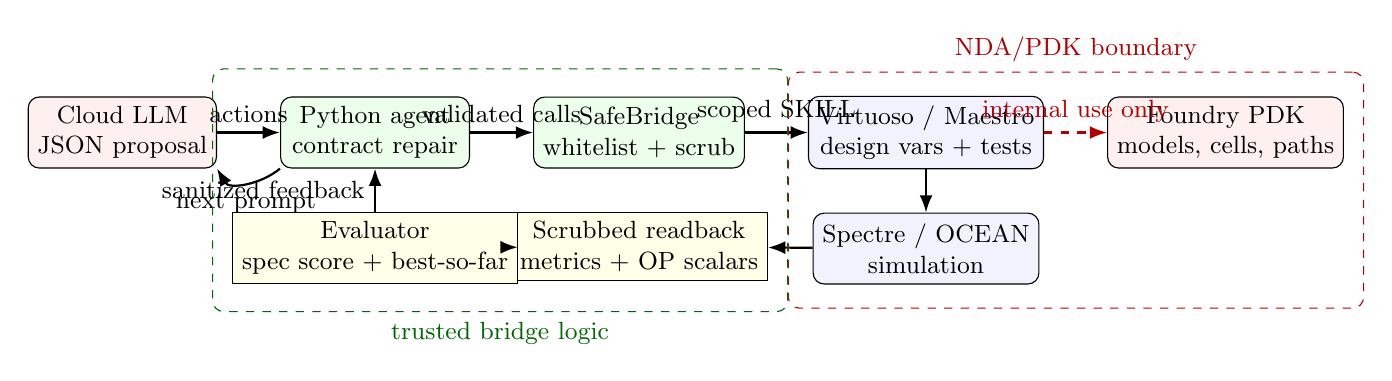
\begin{tikzpicture}[
  font=\small,
  node distance=0.55cm and 0.8cm,
  block/.style={draw, rounded corners, align=center, minimum height=0.9cm,
    minimum width=2.2cm, fill=blue!5},
  safe/.style={draw, rounded corners, align=center, minimum height=0.9cm,
    minimum width=2.4cm, fill=green!8},
  warn/.style={draw, rounded corners, align=center, minimum height=0.9cm,
    minimum width=2.3cm, fill=red!6},
  data/.style={draw, align=center, minimum height=0.75cm, minimum width=2.0cm,
    fill=yellow!10},
  arr/.style={-{Latex[length=2.2mm]}, thick}
]

\node[warn] (llm) {Cloud LLM\\JSON proposal};
\node[safe, right=of llm] (agent) {Python agent\\contract repair};
\node[safe, right=of agent] (bridge) {\bridge\\whitelist + scrub};
\node[block, right=of bridge] (maestro) {Virtuoso / Maestro\\design vars + tests};
\node[block, below=of maestro] (spectre) {Spectre / OCEAN\\simulation};
\node[data, below=of bridge] (readback) {Scrubbed readback\\metrics + OP scalars};
\node[data, below=of agent] (score) {Evaluator\\spec score + best-so-far};
\node[warn, right=of maestro] (pdk) {Foundry PDK\\models, cells, paths};

\draw[arr] (llm) -- node[above]{actions} (agent);
\draw[arr] (agent) -- node[above]{validated calls} (bridge);
\draw[arr] (bridge) -- node[above]{scoped SKILL} (maestro);
\draw[arr] (maestro) -- (spectre);
\draw[arr] (spectre) -- (readback);
\draw[arr] (readback) -- (score);
\draw[arr] (score) -- node[left]{sanitized feedback} (agent);
\draw[arr] (agent.south west) to[out=220,in=300] node[below]{next prompt} (llm.south east);
\draw[arr, dashed, red!70!black] (maestro) -- node[above]{internal use only} (pdk);

\node[draw, dashed, red!70!black, rounded corners, fit=(maestro)(spectre)(pdk),
  inner xsep=0.25cm, inner ysep=0.3cm, label={[red!70!black]above:NDA/PDK boundary}] {};
\node[draw, dashed, green!40!black, rounded corners, fit=(agent)(bridge)(readback)(score),
  inner xsep=0.25cm, inner ysep=0.35cm, label={[green!40!black]below:trusted bridge logic}] {};

\end{tikzpicture}
}%
\caption{Precise \framework{} data flow. The cloud LLM receives JSON actions
and scrubbed observations only. PDK content is referenced inside Cadence and
Spectre but is not serialized into model-visible feedback.}
\label{fig:architecture}
\end{figure*}

\subsection{Safety boundary}

The framework assumes that a cloud LLM provider is curious-but-passive: it can
observe prompts and returned tool results, and it may emit adversarial tool
arguments, but it does not compromise the local operating system or the Cadence
process. Under this model, the protected assets are PDK model contents,
foundry-specific identifiers, proprietary cell/library names beyond the
allowed project scope, user paths, license paths, API keys, and raw simulator
state. The allowed feedback is intentionally narrower: scalar metrics, bounded
waveform summaries, anonymized topology intent, internal node voltages under
safe aliases, and selected device operating-point scalars such as
\metric{id}, \metric{gm}, \metric{gds}, \metric{vgs}, \metric{vds},
\metric{vth}, \metric{vov}, \metric{cgs}, and \metric{cgd}.

The bridge enforces this boundary in four places. First, project specs define
the design variables that the LLM may edit. Second, Python validates
identifier names, numeric values, analysis names, output expressions, and SKILL
entry points before a command reaches Virtuoso. Third, SKILL wrappers on the
Cadence side expose only scoped read and write APIs, rather than arbitrary
database access. Fourth, every return path is scrubbed for paths, foundry-like
tokens, model identifiers, and unsafe strings before the text is reinserted
into the LLM conversation.

\subsection{Maestro setup and writeback}

\framework{} treats Maestro setup as part of the reproducible experiment, not
as manual GUI state. A setup recipe can enable analyses, create output
metrics, define specs, set design variables, and verify that the requested
state landed under the target test row. This was necessary in practice because
AC and DC outputs need different expression families, and because model
comparison is only meaningful when every run starts from the same documented
state. The writeback path records whether test-scoped variables were actually
written; this matters for analog tasks because a visually open Maestro session
can still fail to accept writes if the wrong setup database handle is used.

\section{Benchmark Protocol}
\label{sec:protocol}

\subsection{Tasks}

The LC-VCO task uses a 20 GHz nominal operating point with the control voltage
fixed at 0.4 V for the nominal point and swept over [0.1, 0.7] V for the
tuning curve. The pass condition combines nominal oscillation frequency,
differential swing, common-mode level, duty cycle, startup behavior, current,
monotonicity, and tuning-curve metrics. This task stresses oscillator
simulation, transient startup, swept metrics, and the need to keep design
variables physically plausible.

The op-amp task uses a differential AC/DC testbench with common-mode input
stimulus, output load capacitance, and a two-stage fully differential op-amp
with common-mode feedback. The hard-pass gain target is
$A_0 > 50$ dB, and the unity-gain bandwidth target is above 100 MHz. DC output
and common-mode constraints are included in the Maestro output setup, although
the current benchmark table emphasizes the two stable scalar metrics that were
consistently read back across all runs: \metric{A0\_diff\_db} and
\metric{UGB\_Hz}.

\begin{table}[t]
  \centering
  \caption{Benchmark tasks and pass metrics used in the initial TODAES draft.}
  \label{tab:tasks}
  \begin{tabularx}{\linewidth}{l X X}
    \toprule
    Task & Main metrics & Stress mode \\
    \midrule
    LC-VCO & $f_{osc}$ near 20 GHz, swing, common mode, duty cycle,
    startup, current, monotonic tuning, $K_{VCO}$ & transient oscillator
    startup plus 7-point swept tuning curve \\
    Op-amp & $A_0>50$ dB, UGB $>100$ MHz, DC output/common-mode checks &
    differential AC/DC biasing, compensation, CMFB interaction \\
    \bottomrule
  \end{tabularx}
\end{table}

\subsection{Model comparison protocol}

Each model is evaluated from the same reset state. For the op-amp, all
non-stimulus sizing variables are initialized to one, while stimulus variables
use the differential AC preset: common-mode input 0.4 V, differential AC
magnitude 0.5, positive input phase 0 degrees, and negative input phase
180 degrees. For the LC-VCO, the control voltage is not treated as an
optimization knob; it is fixed by the nominal and sweep definitions. The
iteration budget is 15 unless otherwise specified. A run is counted as
\pass{} only if all hard-pass metrics are satisfied before the budget ends.

The main tables report eleven matched model checkpoints. The same model set is
used for the op-amp and LC-VCO tasks so that cross-task comparisons are not
confounded by different endpoint coverage.

\section{Results}
\label{sec:results}

\subsection{Overall outcome}

The two tasks expose different difficulty profiles. LC-VCO sizing is easier
for the current framework once the swept metric path is stable: 8 of 11 models
pass, with successful runs requiring two to six iterations. Op-amp sizing is
harder: 6 of 11 models pass, and several failing runs still find high-bandwidth
but low-gain points, suggesting that the loop can optimize a visible metric
while missing the coupled biasing and compensation tradeoff required for
differential gain.

\begin{table*}[t]
  \centering
  \caption{Eleven-model LC-VCO tuning-curve benchmark. All runs start from the
  same documented reset state and use a 15-iteration budget.}
  \label{tab:lcvco}
  \footnotesize
  \begin{tabular}{l c r r r r l}
    \toprule
    Model & Outcome & Iter. & Time (s) & $f_{osc}$ (GHz) & Range (GHz) & Failure reason \\
    \midrule
    claude-opus-4-8   & \pass & 4  & 1434.6 & 20.204 & 0.827 & -- \\
    claude-sonnet-4-6 & \pass & 6  & 1666.6 & 20.112 & 0.858 & -- \\
    claude-haiku-4-5  & \fail & 5  & 1110.0 & --     & --    & runner ended before final result \\
    gpt-5.5           & \pass & 3  & 1399.8 & 20.137 & 0.846 & -- \\
    gpt-5.4-mini      & \fail & 15 & 4431.4 & 19.616 & 1.839 & max\_iter \\
    kimi-k2.5         & \pass & 5  & 2476.6 & 20.426 & 0.938 & -- \\
    minimax-m2.7      & \pass & 5  & 1735.6 & 19.634 & 0.937 & -- \\
    mimo-v2.5-pro     & \pass & 6  & 3380.3 & 20.024 & 0.925 & -- \\
    deepseek-v4-pro   & \pass & 2  & 1505.0 & 19.601 & 0.906 & -- \\
    deepseek-v4-flash & \pass & 5  & 2192.9 & 19.987 & 0.918 & -- \\
    gemini-2.5-pro    & \fail & -- & 35.8   & --     & --    & llm\_error \\
    \bottomrule
  \end{tabular}
\end{table*}

\begin{table*}[t]
  \centering
  \caption{Eleven-model op-amp AC/DC benchmark using the same model set as the
  LC-VCO benchmark.}
  \label{tab:opamp}
  \footnotesize
  \begin{tabular}{l c r r r r l}
    \toprule
    Model & Outcome & Iter. & Time (s) & $A_0$ (dB) & UGB (MHz) & Failure reason \\
    \midrule
    claude-opus-4-8   & \pass & 1  & 74.4   & 52.20  & 1707.79 & -- \\
    claude-sonnet-4-6 & \fail & 15 & 1598.2 & 47.18  & 276.74  & max\_iter \\
    claude-haiku-4-5  & \fail & 15 & 1073.0 & -62.94 & --      & max\_iter \\
    gpt-5.5           & \pass & 4  & 450.6  & 51.58  & 212.00  & -- \\
    gpt-5.4-mini      & \fail & 15 & 917.1  & -76.81 & --      & max\_iter \\
    kimi-k2.5         & \pass & 3  & 835.4  & 50.11  & 1543.39 & -- \\
    minimax-m2.7      & \fail & 15 & 1503.7 & 16.90  & 3864.13 & max\_iter \\
    mimo-v2.5-pro     & \pass & 4  & 1386.5 & 50.94  & 121.13  & -- \\
    deepseek-v4-pro   & \pass & 2  & 322.7  & 50.88  & 841.37  & -- \\
    deepseek-v4-flash & \pass & 15 & 1412.3 & 52.73  & 896.32  & -- \\
    gemini-2.5-pro    & \fail & 1  & 173.9  & -24.23 & 4645.97 & llm\_error \\
    \bottomrule
  \end{tabular}
\end{table*}

\subsection{Cross-task observations}

First, passing LC-VCO does not imply passing op-amp. MiniMax-M2.7 passes the
LC-VCO sweep but fails the op-amp gain target after 15 iterations, while
Claude Sonnet passes LC-VCO but stalls at 47.18 dB on the op-amp. This
supports treating analog agent evaluation as a multi-topology benchmark rather
than a single-circuit leaderboard.

Second, the op-amp failures are informative rather than random. Several failed
runs produce very high UGB values but insufficient or negative low-frequency
gain. This is a recognizable analog-design failure mode: the model has found a
fast biased point or a misbiased point, but not the operating-region and
compensation balance needed for gain. The framework changes this from an
opaque model failure into a debuggable trace because the LLM-visible feedback
contains AC metrics, DC readback, topology intent, and operating-point scalars.

Third, tool-protocol reliability is part of model quality in an EDA agent. Some
runs fail through \metric{llm\_error}, \metric{contract\_violation}, or runner
termination rather than through circuit metrics alone. The benchmark therefore
reports both analog success and tool-loop failure reason. This is important
because a model that can reason about circuits but cannot reliably emit the
contracted JSON action is not deployable as a closed-loop EDA agent.

\section{Ablation and Failure Analysis}
\label{sec:ablation}

The current draft separates completed evidence from planned ablations. The
completed evidence shows that the full feedback path can support successful
optimization on two circuits. The planned ablations will quantify which parts
of the feedback are necessary:
\begin{enumerate}
  \item \textbf{No topology intent}: remove the first-turn topology summary and
  test whether models still identify the input pair, tail current, load, CMFB,
  and output stage.
  \item \textbf{No operating-point scalars}: remove device-level current,
  transconductance, conductance, voltage, threshold, overdrive, and capacitance
  summaries and measure whether op-amp bias failures increase.
  \item \textbf{No best-so-far writeback}: leave the final point in Maestro
  after max-iteration failure and measure how often the saved state regresses.
  \item \textbf{Loose natural-language protocol}: allow free-form model output
  rather than strict JSON action repair and measure contract failures.
  \item \textbf{Manual Maestro setup}: compare recipe-based setup writeback
  against manually prepared GUI state to measure reproducibility failures.
\end{enumerate}

The failure taxonomy used for the current runs has five buckets:
\begin{enumerate}
  \item \textbf{Metric miss}: simulation completes but the hard-pass metric is
  not met, such as op-amp gain below 50 dB.
  \item \textbf{Bias or operating-region miss}: the run produces high bandwidth
  or oscillation but the underlying transistor operating point is implausible.
  \item \textbf{Contract failure}: the model fails to emit valid JSON or emits
  unsupported structural edits.
  \item \textbf{Tool/readback failure}: simulation or PSF/OCEAN readback does
  not produce the requested scalar results.
  \item \textbf{Runner failure}: the benchmark harness terminates before a
  final result can be parsed.
\end{enumerate}

\section{Reproducibility and Security Audit}
\label{sec:repro}

The reproducibility package has two layers. The public layer contains the
agent code, project specifications, Maestro setup recipes, scrubbed transcripts,
benchmark summaries, and leak-check scripts. The private layer is supplied by
the user: a licensed Virtuoso/Maestro/Spectre installation, an opened Maestro
session for the target testbench, and a foundry PDK that remains local. This
split is intentional. A reviewer can inspect the safety mechanism and replay
scrubbed benchmark evidence without receiving the PDK.

The security audit checks for three classes of leakage. First, source-level
leak checks scan the repository for private paths, API keys, remote host names,
and foundry-shaped tokens. Second, bridge-level tests verify that schematic
readback, operating-point readback, OCEAN result generation, and Maestro
writeback return only whitelisted fields. Third, transcript-level checks verify
that the exact text sent back to the LLM does not include PDK model names,
absolute paths, or hidden reasoning content that bypasses the scrubber.

\todo{Before submission, regenerate the P0 leak report and cite the exact
script output, commit hash, and benchmark artifact manifest.}

\section{Discussion}
\label{sec:discussion}

\framework{} deliberately optimizes a conservative surface: sizing variables,
analysis setup, outputs, and specs. It is not a topology-synthesis system, and
it does not claim that cloud LLMs should see raw netlists or model cards. This
limited scope is a strength for industrial adoption because it matches a common
designer workflow: keep the schematic and PDK local, let an assistant propose
numeric sizing moves, and use the simulator as the source of truth.

The main limitation is benchmark breadth. LC-VCO and op-amp already expose
different failure modes, but a full TODAES version should add more topologies
or more seeds per topology. The second limitation is that safety and usefulness
trade off against each other. Too little feedback leaves the model guessing;
too much feedback risks leaking design or PDK information. Our current design
suggests that sanitized topology intent plus numeric operating-point scalars
is a useful middle ground, but the ablation section must quantify that claim.

Finally, model comparisons should not be interpreted as permanent rankings.
Provider endpoints, context behavior, tool-call discipline, and pricing change
over time. The durable contribution is the benchmark method: fixed reset,
fixed Maestro setup, fixed spec, fixed feedback schema, and logged failure
reason. The reported tables are a snapshot generated under that method.

\section{Conclusion}
\label{sec:conclusion}

This paper presented \framework, an NDA-safe closed-loop framework for
LLM-driven analog circuit sizing through industrial Virtuoso/Maestro flows. The
framework combines scoped SKILL access, PDK/path/model scrubbing, Maestro
setup recipes, AC/DC and swept-metric readback, operating-point summaries,
strict JSON contracts, and best-so-far writeback. In matched eleven-model
benchmarks, 8 of 11 models pass the LC-VCO tuning-curve task and 6 of 11 pass
the op-amp AC/DC task. These results support the paper's central claim: cloud
LLMs can be evaluated and used in real analog EDA loops without exposing raw
PDK content, but their reliability must be measured at the level of complete
tool-loop behavior rather than standalone text reasoning.

\section*{Draft Self-Review}

\textbf{Contribution.} The draft foregrounds the safety-bounded EDA system and
matched benchmark protocol, not a weak ``first LLM analog design'' claim.

\textbf{Clarity.} The terminology is stable: \framework{} is the whole agent,
\bridge{} is the safety bridge, and Maestro writeback is the scoped EDA state
update path.

\textbf{Experimental strength.} The main result tables are real current CSV
data, but the ablation section is still a plan and must be run or clearly
marked as future work before submission.

\textbf{Evaluation completeness.} Two circuits are enough for a serious first
draft, but additional seeds or one more topology would make the TODAES story
stronger.

\textbf{Method soundness.} The benchmark protocol uses matched resets and fixed
model sets; the next revision should add exact commit hashes, leak-check logs,
and artifact manifests.

\bibliographystyle{ACM-Reference-Format}
\bibliography{../refs}

\end{document}
